\newpage
\section{Morfeas ISO Channel Linker}
The ``Morfeas ISO Channel Linker" is an utility made to create ISO channels and link them with sensors.
It's can be accessed by the Morfeas WEB front page from the button with the anchor (
\includegraphics[height=.125in]{../art/anchor.png}) symbol.
At figure \ref{fig:ISOChannel_linker} shown an example of the ``Morfeas ISO Channel Linker" utility.

\begin{figure}[h]
\centering
	\fbox{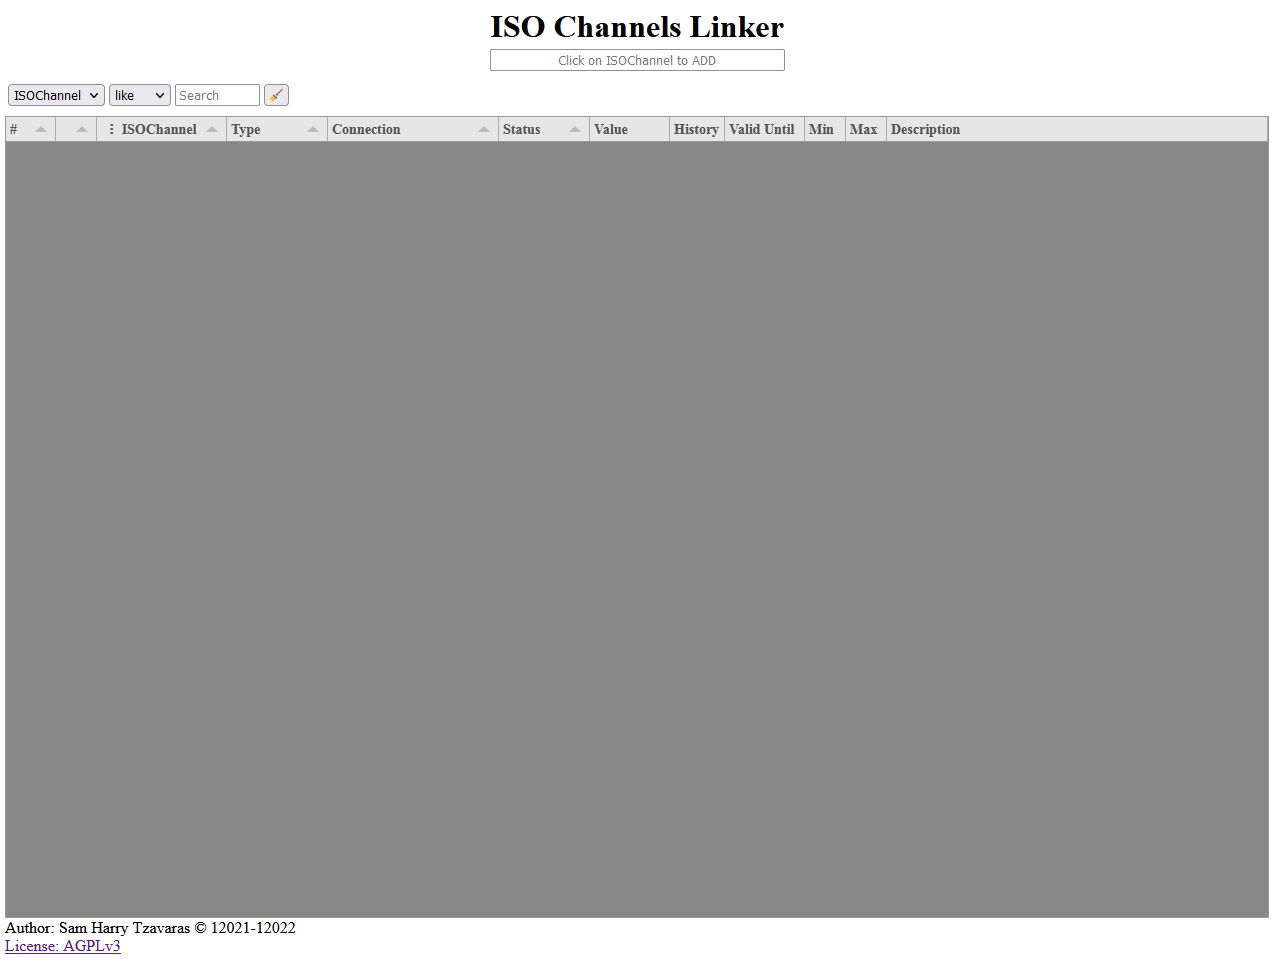
\includegraphics[width=3in,angle=0]{../art/Morfeas_web_if/Morfeas_WEB_ISOChannel_linker.png}}
	\caption{Morfeas ISO Channel Linker Utility}
	\label{fig:ISOChannel_linker}
\end{figure}
\noindent
The utility window split in three sections: the status bar, the filters section, and the ISO Channels table.\\

The status bar show the last update date if at least one channel exist,
or a message that informing the user to add channel(s).\\

The filter section, is filtering the ISO channels table, accordingly to the command from the user.
The filtering command is specified from the two drop-down lists and the text input field.
The first drop-down is selecting the column that the filtering will applied.
The second drop-down select the filter type; for most of the columns (except ``Min" and ``Max")
is ``like" and ``regex". The ``Like" filter type is filter and show all the elements in the specified column,
that contains the word in the search field, and similarly the ``regex" the fields that agree with the regular expression phrase.
For columns ``Min" and ``Max" the filter type become numerical compare.
The button with the broom is cleaning the filter.\\

